\documentclass[11pt,letterpaper,oneside,openright]{book}

\usepackage[spanish]{babel}
\usepackage[utf8]{inputenc} 
\usepackage{lmodern}
\usepackage[T1]{fontenc}

\usepackage{textcomp}
\usepackage[pdftex]{hyperref}
\usepackage{multirow}
\usepackage{booktabs}
\usepackage{graphicx}
\usepackage{tikz}
% \usepackage{bordermatrix}

% \usepackage{microtype}
% \usepackage{shortvrb}

% \usepackage{tabularx}


%%%%%%%%%%%%%%%%%
% PARA HACER LA PRUEBA
%%%%%%%%%%%%%%%%%
% \usepackage{nicefrac}
% \usepackage[pdftex]{hyperref}
% \usepackage{anysize}
% \usepackage{fancyhdr}
% \usepackage{subfigure}
% \usepackage{pstricks}
% \usepackage{tabulary}
% \usepackage{type1cm}
% \usepackage{url}

% \usepackage{multirow}
% \usepackage{booktabs}

% \usepackage{subfigure}
% \usepackage{graphicx}

% \usepackage{bm}
%%%%%%%%%%%%%%%%%%%%%%%%%%%%%%%%%%%%%%

% \usepackage[bookmarks]{}
% \usepackage[bookmarks,colorlinks]{hyperref}


\graphicspath{{images/}}
% \renewcommand{\arraystretch}{1.5}
% \usepackage{hyperref}
\hypersetup{colorlinks,%
            citecolor=black,%
            filecolor=black,%
            linkcolor=black,%
            urlcolor=black}

% \usepackage[charter]{mathdesign}

\title{Red Social con Geo-Localizaci\'on de lugares\\ basado en tecnolog\'ia Ruby on Rails}
\author{Edmundo Figueroa Herbas}
\date{\today \ }

\begin{document}
% \include{title-page}
\frontmatter
  \maketitle
  \tableofcontents

\mainmatter
  \chapter{Introducci\'on} % (fold)
\label{cha:introduccion}

  La ciudad cuenta con lugares turísticos o de interés y es fácil perderse al no 
  tener conocimiento del nombre de las calles, movilidades que circulan por la 
  zona o directamente no saber a dónde ir, un turista que viene por primera vez 
  tiene el deseo de conocer un restaurant criollo   o el comprador que necesita 
  localizar el cajero automático mas cercano, toda esta información es difícil de 
  conocer o conseguir ya que la gente del lugar no conoce el destino deseado o  
  pueden existir muchas razones por lo cual es fácil perderse y  el tiempo es uno 
  de los recursos  más preciados en la actualidad.\\

  Los lugares turísticos son de especial interés por parte de gente que viene a 
  conocer la ciudad y es una gran fuente de ingreso por parte de gente del lugar 
  como también de empresas que se dedican al turismo, lo más importante el 
  turista es contar con información confiable del lugar que va a visitar, esta 
  información es un gran aliciente para el crecimiento de esta industria.
   % (sin chimeneas).

  \section{Antecedentes} % (fold)
  \label{sec:antecedentes}
    Actualmente existen blogs o redes sociales dedicadas al intercambio de 
    información, pero  la gran mayoría se basa solamente en intercambiar opciones 
    o gustos sobre determinados lugares, o se centran exclusivamente en los 
    lugares de más alta afluencia turística por ejemplo: el salar de Uyuni, el 
    lago Titikaka o por fechas festivas por ejemplo el carnaval de Oruro.\\ 

    Alguno de estos portales son  exploroo.com, dopplr.com, tripwolf.com, que 
    ofrecen servicios como ser estado del tiempo, búsqueda de hoteles, con 
    opciones como poder programar una guía turística personalizada, pero con la 
    desventaja que para nuestro país la información es tan escasa como ambigua, 
    estos portales son de gran utilidad para llegar al destino pero no existe la 
    información adecuada para los usuarios que quieran moverse  y conocer la ciudad.
  % section antecedentes (end)

  \section{Descripción del problema} % (fold)
  \label{sec:desc_probl}
    En una ciudad o región donde existen muchos lugares de interés para propios o 
    extraños siempre falta una guía actualizada que nos permita movernos o tomar 
    decisiones, las guías disponibles son generalmente impresas y solo llevan un 
    registro de los lugares más destacados o de aquellos que pagan el derecho de 
    aparecer en la guía, además que no se tiene la certeza si la información  es 
    actual. \\

    En una ciudad los cambios se dan de un día para otro, locales que cierran, 
    calles que cambian de dirección,  rutas de movilidades (trufis, taxitrufis) 
    que son modificadas o creadas, donde tener información actual es primordial.\\

    Actualmente la Universidad Mayor de San Simon, no cuenta con un mapa
    actualizado de las locaciones  internas, y para los estudiantes nuevos o 
    personas que necesitan hacer algun tramite, se hace difícil el movilizarse
    dentro del Campus Universitario. 
    % por lo tanto es muy importante el contar 
    % con algun tipo de guia que nos permita recorrer y visitar el campus universitario.
  % section desc_probl (end)

  \section{Objetivo general} % (fold)
  \label{sec:objetivo_general}
    \begin{quote}
      Construir un Prototipo de Red Social para localización de lugares con 
      tecnología Ruby on Rails (RoR).
    \end{quote}
  % section objetivo_general (end)

  \section{Objetivos Específicos} % (fold)
  \label{sec:obj_especificos}
    \begin{itemize}
      \item Analizar el framework Ruby on Rails para el desarrollo de aplicaciones web2.0
      \item Proponer 3 patrones web2.0 aplicables al problema.
      \item Implementar 3 Patrones web2.0 con tecnología RoR.
      \item Analizar y construir un modulo con características de geo-localización para la Red Social.
    \end{itemize}
  % section obj_especificos (end)

  \section{Justificación:} % (fold)
  \label{sec:justificacion}
    La gran acogida de la población en general por las redes sociales, hace 
    hincapié en el desarrollo de un sistema de  que sea ágil y eficiente en el 
    manejo de información, ayudándose en las tecnologías  presentes en la web2.0 y 
    que tenga una gran cobertura, mediante el cual  ayude a conocer la ciudad  o 
    decidir al lugar donde nos podemos dirigir indicando una ruta optima.

  % section justificacion (end)
% chapter introduccion (end)


  
  
  




% Metodología:
% Agile Unified Process (AUP) es una versión simplificada de Rational  Proceso 
% Unificado  (RUP). 

% Fases del ciclo de desarrollo
%   Principio: El objetivo es  identificar el alcance inicial del proyecto y una 
%   arquitectura potencial del sistema.
  
%   Elaboración: El objetivo es confirmar la idoneidad de la arquitectura del sistema.
%   Construcción: El objetivo es desarrollar software funcional dentro de un sistema regular e incremental periódicamente que mire las necesidades de las partes interesadas.
%   Transición: El objetivo es validar y desplegar el sistema en su entorno de producción.
% Las disciplinas del ciclo de desarrollo se llevan de manera iterativa y son 
% las siguientes
%   Modelo: El objetivo de esta disciplina es entender el negocio de la organización, el dominio del problema que se ocupa el proyecto, y determinar una solución viable para hacer frente al dominio del problema.
%   Aplicación: El objetivo de esta disciplina es transformar el modelo de su (s) en el código ejecutable y para llevar a cabo un nivel básico de las pruebas, en las pruebas de unidad en particular.
%   Prueba: El objetivo de esta disciplina consiste en realizar una evaluación objetiva para asegurar la calidad. Esto incluye encontrar defectos, validar que el sistema funcione como está previsto, y verificar que se cumplan los requisitos.
%   Implementación: El objetivo de esta disciplina es el plan para la entrega del sistema y para ejecutar el plan para que el sistema a disposición de los usuarios finales.
%   Gestión de la Configuración: El objetivo de esta disciplina consiste en administrar el acceso a artefactos de su proyecto. Esto incluye no sólo el seguimiento de versiones de los artefactos a través del tiempo, sino también el control y la gestión de los cambios a los mismos.
%   Gestión de Proyectos: El objetivo de esta disciplina es dirigir las actividades que lleva a cabo en el proyecto. Esto incluye la gestión de riesgos, la dirección de personas (la asignación de tareas, seguimiento de los progresos, etc.), y coordinar con la gente y los sistemas fuera del alcance del proyecto para asegurarse de que se entregue a tiempo y dentro del presupuesto.
%   Para el Medio Ambiente: El objetivo de esta disciplina es apoyar el resto de los esfuerzos por garantizar que el proceso, la orientación adecuada (las normas y directrices), y herramientas (hardware, software, etc.) están disponibles para el equipo según sea necesario.
% % Fig. Ciclo de vida del Proceso Unificado Ágil   
  \chapter{Marco Referencial} % (fold)
\label{cha:marco_referncial}

  % \section{Introducci\'on} % (fold)
  % \label{sec:Introduccion}
    
  % % section Introduccion (end)

  \section{Ruby on Rails} % (fold)
  \label{sec:ruby_on_rails}
    Ruby on Rails es un framework dise\~nado para desarrollar aplicaciones web, 
    y está construido sobre el lenguaje de programación Ruby, Ruby  fue creado
    alrededor de 1993 por Yukihiro ``Matz'' Matsumuto de Jap\'on, y liberado al 
    público en 1995, y desde entonces fue ganando  popularidad y 
    reputaci\'on gracias al aporte de una gran variedad de programadores, que 
    realzan la sintaxis elegante y el código limpio que se genera, Ruby es un 
    lenguaje de programación multiparadigma ya que implementa programaci\'on 
    Orientado a Objetos, programaci\'on Funcional así como también 
    programaci\'on Imperativa. \\

    Ruby on Rails fue creado en el 2004 por David Heinemeier Hansson durante el desarrollo de Basecamp, una aplicación de gesti\'on de proyectos, y una vez que se necesitó para otros proyectos, el equipo de desarrollo extrajo el core de funcionalidad el cual fue presentado al público en julio del 2004 con el nombre de Ruby on Rails, como proyecto Open Source bajo una licencia MIT, desde entonces tuvo un gran  crecimiento impulsado por la comunidad de usuarios que continuamente están desarrollando nuevas características, limpiando bugs y creando gemas\footnote{ Los plugins o complementos, en el lenguaje Ruby son llamados \textbf{gemas}}. La última versión de Rails es la 3.2 publicado en enero del 2012 y actualmente está en su revisi\'on 3.2.8 presentado en agosto del 2012,  demostrando que el equipo de desarrollo de Rails esta trabajando constantemente en mejorar este framework que actualmente está entre los mejores en desarrollo web.\\
     % y se prevee que la versión 4 de Rails sea lanzada a finales del 2012, pero no  \\
    % y para el proyecto se utilizó la versión 3.2.3

    El núcleo de funcionalidad de Rails es un conjunto de funciones llamadas \emph{Railties}:
    \begin{description}
      \item[Active Record] Es una implementaci\'on del patrón
        Object-Relational Mapping(ORM), que mapea las tablas de la Base de datos relacional en clases, filas en objetos y 
        columnas en atributos de los objetos.   
      \item[Active Support] Es el componente de Rails responsable de proporcionar extensiones del lenguaje Ruby, utilitarios y funciones primordiales a la hora de realizar cualquier tarea en el desarrollo de la aplicaci\'on.  
      \item[Action Mailer] Permite enviar correo electrónico (email) desde la aplicaci\'on usando un  modelo y vistas.
      \item[Action Pack] Es el responsable de manejar y responder los request del navegador web. Provee las herramientas para el \textbf{routing}, define los \textbf{controladores}, y genera las respuestas renderizando las \textbf{vistas}. En resumen, Action Pack maneja las capas de la vista y el controlador del paradigma MVC.  
    \end{description}
    Otra de las características de Rails es la facilidad para escribir Pruebas, en realidad Rails sugiere el modelo de Desarrollo guiado por Pruebas(TDD\footnote{Test-Driven Development, por sus siglas en Inglés}), que consiste en 3 pasos
    \begin{enumerate}
      \item \textbf{Rojo}, la prueba falla
      \item \textbf{Verde}, la prueba pasa
      \item \textbf{Refactorizar}, limpiar el código 
    \end{enumerate}
    Para este proceso, Rails ofrece primeramente el módulo Test::Unit, pero también se pueden encontrar variadas herramientas para llevar a cabo está tarea.\\

    Ruby on Rails es un framework MVC, que implementa los principios REST, No te Repitas\footnote{DRY, Don't Repit Yourself}, Convenci\'on sobre Configuraci\'on, estas características de Rails están explicadas con mayor detalle en el capítulo \ref{cha:ruby_on_rails_y_patrones_web_2_0}.


  % section ruby_on_rails (end)

  \section{Base de Datos} % (fold)
  \label{sec:base_de_datos}

    En una aplicación web es necesario alguna forma de persistencia de datos, en especial si se están usando datos complejos y en gran cantidad, para realizar está tarea, la base de datos es un factor primordial.
    Rails maneja la base de datos mediante  un ORM, por lo tanto la base de datos que se utilice no es tan excluyente, en este caso se utilizó  \emph{PostgreSQL} como base de datos relacional.\\

    \subsection{PostgreSQL} % (fold)
    \label{sec:postgres}

      PostgreSQL es un sistema de gestión de bases de datos objeto-relacional, Open Source y distribuido bajo licencia BSD. 
      PostgreSQL utiliza un modelo cliente/servidor y usa multiprocesos en vez de multihilos para garantizar la estabilidad del sistema. Un fallo en uno de los procesos no afectará el resto y el sistema continuará funcionando.
      La última versi\'on de PostgreSQL es la 9.2, su desarrollo comenz\'o hace más de 16 años, y cuenta con una gran comunidad que aporta con el desarrollo, testeo de nuevas versiones.
      PostgreSQL  está considerada como una de los mejores \emph{Sistemas de gesti\'on de bases de datos}, es muy completo y está muy bien documentado\footnote{ http://www.postgresql.org/docs/9.2/static/}. 
      Entre sus características se pueden nombrar las siguientes.
      \begin{itemize}
        \item Es una base de datos 100\% ACID\footnote{  ACID es un acrónimo de Atomicity, Consistency, Isolation and Durability}
        \item Integridad referencial
        \item Replicación asincrónica/sincrónica
        \item Múltiples métodos de autentificación
        \item Disponible para Linux y UNIX en todas sus variantes
        \item Funciones/procedimientos almacenados
        \item Soporte a la especificaci\'on SQL
      \end{itemize}

      Personalmente se escogió trabajar con  PostgreSQL como DBMS
      porque cuenta con una extensa documentación,  y gracias a su caracter ``Open Source'', y su gran flexibilidad en poder definir nuevos tipos de datos, 
      se hace posible que empresas como \textbf{Refractions Research} puedan crear recursos como PostGIS, necesario para trabajar con datos geográficos \'o espaciales.

      % Entre sus principales  características se puede nombrar que es
      % \footnote{ DBMS, DataBase Management System}
      % y durante este tiempo, estabilidad, potencia, robustez, facilidad de administración e implementación de estándares han sido las características que más se han tenido en cuenta durante su desarrollo. PostgreSQL funciona muy bien con grandes cantidades de datos y una alta concurrencia de usuarios accediendo a la vez a el sistema.

    % section postgres (end)

    \subsection{PostGis} % (fold)
    \label{sec:postgis}

      PostGIS es un módulo  que a\~nade soporte de objetos geográficos al DBMS PostgreSQL, convirtiéndola en una base de datos espacial para su utilización en un Sistema de Informaci\'on Geografica(SIG\footnote{ Es bastante común utilizar el acrónimo en Inglés, Geographic Information System (GIS), de hay viene el término de PostGIS = Postgres + GIS}).

      El desarrollo de PostGIS está a cargo de \textbf{Refractions Research}, está liberada con la \emph{Licencia pública general de GNU}, declarandola como software libre y lo protege de cualquier intento de apropiaci\'on.\\

      PostGIS implementa la especificaci\'on ``SFSQL'' (Simple Features for SQL, define los tipos y funciones que necesita implementar cualquier base de datos espacial) de la OGC (Open Geospatial Consortium, es un consorcio internacional, formado por un conjunto de empresas, agencias gubernamentales y universidades, dedicado a desarrollar especificaciones de interfaces para promover y facilitar el uso global de la información espacial).\\

      PostGIS al igual que PostgreSQL tiene una documentaci\'on bastante extensa, y cuenta con equipo de desarrollo que continuamente va sacando nuevas versiones, actualmente se encuentra la versi\'on 2.0.1, pero para el desarrollo de la aplicaci\'on se hizo uso de la versi\'on 1.5.5.

      PostGIS es gratis, pero no por ello es una herramienta de baja calidad, al contrario se la considera una herramienta de nivel empresarial, y muchas instituciones la est\'an usando de manera exitosa\footnote{ http://www.postgis.org/documentation/casestudies/}, aparte de numerosas aplicaciones \\

      Manejar los datos geográficos con PostGIS es sencillo y muy eficiente, por está raz\'on se utilizó está herramienta, pero para conseguir la ruta óptima entre 2 puntos se necesitaba el uso del algoritmo de Dijkstra y para PostGIS existe el módulo \textbf{PgRouting}, que tiene implementado este algoritmo.
      
      \subsubsection{pgRouting} % (fold)
      \label{sec:pgrouting}
        pgRouting es una extensi\'on  de  PostGIS para proveer funcionalidades de ruteo espacial. pgRouting es un desarrollo posterior de pgDijkstra y actualmente está siendo mantenido por Georepublic, la última versi\'on estable es la 1.05, y es la que fue usada para desarrollar el sistema.\\

        Las ventajas del ruteo en la base de datos son:
        \begin{itemize}
          \item Los datos y atributos pueden ser modificados desde varios clientes, como Quantum GIS y uDig a través de JDBC, ODBC, o directamente usando Pl/pgSQL. Los clientes pueden ser PCs o dispositivos móviles.
          \item Los cambios pueden ser reflejados instantáneamente a través del motor de ruteo. No hay necesidad de hacer cálculos previos.
          \item El parámetro de ``costo'' puede ser calculado dinámicamente a través de SQL y su valor puede provenir de múltiples campos y tablas.
        \end{itemize}

        pgRouting provee funciones para:
        \begin{itemize}
          \item Camino mínimo (Dijkstra): algoritmo de ruteo sin heurística
          \item Camino mínimo (A-Star): routeo para conjunto de datos grandes (con heurística)
          \item Camino mínimo (Shooting-Star): ruteo con restricciones de giro (con heurística)
          \item El problema del viajante (TSP: Traveling Salesperon Problem)
          \item Cálculo de ruta (Isolíneas)
        \end{itemize}
        
        % Uses PostGIS for its geographic data format, which in turn uses OGC’s data format Well Konwn Text (WKT) and Well Known Binary (WKB)
      % section pgrouting (end)
    % section postgis (end)
  % section base_de_datos (end)
% chapter marco_referncial (end)  
  \chapter{Ruby on Rails y patrones Web 2.0} % (fold)
\label{cha:ruby_on_rails_y_patrones_web_2_0}

  \section{Porque usar Ruby on Rails para desarrollar una aplicación web ?} % (fold)
  \label{sec:porque_usar_ruby_on_rails_para_desarrollar_una_aplicacion_web}

    La gran propaganda de Ruby on Rails (RoR) o más sencillamente Rails
    se basa en el rápido desarrollo de aplicaciones web, conocido como agile development.
    Como parte de su construcci\'on, Rails maneja las filosofías \emph{DRY}\footnote{Don’t Repeat Yourself} y \emph{convención sobre configuración}. 

    \begin{description}
      \item[No te repitas(DRY)] según el creador de RoR, \mbox{David} \mbox{Heinemeier} Hansson, 
      significa que cada pieza de conocimiento en un sistema 
      debe ser declarado en un solo lugar.\cite{awdr4e} 
      Esto lo logra gracias al patrón Modelo-Vista-Controlador\footnote{MVC}, 
      y el lenguaje multiparadigma Ruby sobre el cual está construido Ruby on Rails.
      
      \item[Convención sobre configuración] significa que Rails tiene parámetros por 
      defecto para casi todos los aspectos que mantiene unida una aplicación, ya que se logro
      observar que la gran mayoria de aplicaciones web compartian la misma configuraci\'on inicial,
      siguiendo  las convenciones de Rails se llega a simplificar el código escrito en una aplicación, tambi\'en se agiliza el desarrollo ya que no es necesario tomar decisiones sobre características basicas que se necesita implementar.
    \end{description}


    David Heinemeier cita en su libro \cite{awdr4e}, que \emph{“Rails es Ágil porque 
    simplemente la agilidad es parte de su construcción”}.\\

    Se puede analizar esta afirmaci\'on teniendo en cuenta los principios del
     \textbf{manifiesto por el desarrollo ágil de software}\footnote{http://agilemanifesto.org/iso/es/}:
    \begin{itemize}
      \item \textbf{Individuos e interacciones} sobre procesos y herramientas
      \item \textbf{Software funcionando} sobre documentación extensiva
      \item \textbf{Colaboración con el cliente} sobre negociación contractual
      \item \textbf{Respuesta ante el cambio} sobre seguir un plan
    \end{itemize}
    
    Rails se enfoca bastante en conseguir un prototipo funcional en muy poco tiempo 
    y sobre ese prototipo seguir incrementalmente hasta conseguir una aplicacion 
    de calidad.\\
     % en poco tiempo.\\

    Los más grandes obstáculos que se enfrenta una aplicación en el tiempo es el 
    mantenimiento y escalabilidad, actualmente se estima que existen 230,000 websites\cite{web2} 
    desarrolladas sobre RoR %\footnote{Ruby on Rails, tambi\'en se lo puede nombrar \emph{Rails}, \emph{RoR}}, 
    entre ellas se puede nombrar a GitHub, Hulu, Yellow Pages. Son sitios con miles de visitas diarias
    con una alta carga del servidor y son un claro ejemplo de que Rails puede manejar sitios de alto perfil.\\

    Los detractores de Rails sostienen que escalar una aplicación construida 
    sobre RoR es muy difícil pero los defensores argumentan que lo que se 
    tiene que escalar es el código de la aplicación no el framework.\\

    Twitter nació sobre Ruby on  Rails  y no fue hasta que era un servicio usado 
    a nivel mundial y manejaba millones de request por día que empezaron a surgir 
    problemas debido a que Ruby no estaba optimizado para un trabajo muy pesado, 
    según palabras de Alex Payne, Twitter developer, “Ruby es lento”\cite{web3}. 
    Actualmente Twitter migró su backend a Scala, framework basado en Java(que esta mas optimizado que Ruby),
    pero para su front-end no cambian a Rails.\cite{web4}\\
    
    Se puede agregar que Rails es una muy buena opción a la hora de empezar 
    cualquier proyecto web, ya que implementa las herramientas necesarias 
    para un desarrollo ágil, sólido y de calidad respaldado por un modelo 
    de desarrollo basado en pruebas(TDD\footnote{Test Driven Development}), las filosofías DRY y convención sobre configuración.
    y cundo la aplicaci\'on haya crecido y empiecen a aparecer los problemas es 
    decisión de los programadores el ver si mantener el código actual y parchearlo o 
    cambiar de tecnología para mejorar el rendimiento y la experiencia del usuario\\
  % section porque_usar_ruby_on_rails_para_desarrollar_una_aplicacion_web (end)

  \section{Patrones de diseño de la Web 2.0} % (fold)
  \label{sec:patrones_web20}
    Que es la Web2.0 ?,  primeramente  se debe explicar que este término fue acuñado 
    por 1999 para describir paginas web que usaban tecnologias mas alla de las 
    simples estaticas paginas web.\\
    
    No fue hasta que en  el 2004 en la conferencian sobre la Web2.0 que se popularizo este termino, 
    y asi mismo como la Web que evoluciona, la definicion se actualiza con el tiempo, 
    y Tim O’Reilly trato de definirla en su articulo ``\emph{What is Web 2.0}''\cite{web5},
    articulo que se puede considerar como la guia de referencia para cualquier persona que quiera
    entender que es la Web2.0 y sus origenes,
    en un articulo posterior ``\emph{Web 2.0 Compact Definition: Trying Again}''\cite{web9}
    del que se puede extraer la siguiente definici\'on:\\
    \begin{quote}
      “Web 2.0 is the business revolution in the computer industry caused by the move to the
       Internet as a platform, and an attempt to understand the rules for success on that new
       platform. Chief among those rules is this: build applications that harness network
       effects to get better the more people use them.”
       \begin{flushright}
       --Tim O’Reilly
       \end{flushright}
    \end{quote}
    En resumen se puede definir que una aplicación web2.0 es aquella que mejora y crece con la 
    participación activa de sus usuarios.

    \begin{quote}
      “Software que mejora mientras más gente la usa” \cite{web5}
    \end{quote}

    \subsection{Patrones de dise\~no} % (fold)
    \label{sub:patrones_de_diseno}
    

    Un patrón de diseño es una solución general, reusable  y flexible 
    que describe cómo resolver algún problema general en el desarrollo 
    de software, un patrón puede ser usado y modificado segun el problema 
    al cual se esta aplicando.\\

    Se pueden observar los siguientes patrones de dise\~no en la aplicación:
    \begin{itemize}
      \item \textbf{REST}
      \item \textbf{MVC}
      \item \textbf{Mashup}
    \end{itemize}
    % subsection patrones_de_diseno (end)

    \subsection{REpresentational State Transfer (REST)} % (fold)
    \label{sub:rest}
      REST es un término descrito por Roy Fielding en su tesis doctoral ``\emph{Architectural Styles and the design of Network-based Software Architectures}''\cite{web6}, describe estilos arquitectónicos de sistemas interconectados por red.

      REST es un estilo arquitectónico que especifica cómo los recursos van a ser definidos y direccionados, especifica la importancia del protocolo \emph{cliente-servidor-sin estado}, ya que cada request tiene toda la información necesaria para entenderla.\\

      En el contexto de Rails, REST significa que los componentes del sistema por ejemplo los usuarios son modelados como recursos que pueden ser creados, leídos, actualizados y borrados, estas acciones corresponden a las operaciones CRUD (Create, Read, Update, Delete) de las base de datos relacionales  y a los cuatro operaciones fundamentales POST, GET, PUT, DELETE definidos en el  protocolo HTTP.\\

      En Rails el estilo de desarrollo RESTful\footnote{se denomina RESTful a los sistemas que siguen los principios REST} ayuda a determinar acerca de qué controlador y cuál será la acción que se ejecutará, solamente procesando el request HTTP hecho al servidor.\\

      \textbf{GET} es la operación HTTP más común, es usado para leer 
      datos en este caso paginas, se puede leer como ``get a page'', 
      \textbf{POST} es la operación que se usa cuando se ejecuta un formulario, 
      en la convención de Rails \textbf{POST} se usa para crear 
      objetos o recursos, \textbf{PUT} se usa para actualizar objetos, 
      \textbf{DELETE} es usado para borrar objetos.  Los browsers actuales no son capaces 
      de manejar las operaciones \textbf{PUT} y \textbf{DELETE} de forma nativa, 
      por lo que Rails usa un pequeño truco que consiste en declarar el método 
      que se esta enviando en un \emph{hidden field} en el formulario HTML.\\

      Para lograr todo este comportamiento  es necesario declarar, en el archivo 
      que controla las rutas dentro de la aplicación, \textbf{routes.rb}, que el 
      recurso \textbf{user} es \emph{restful}, tal como se muestra en la figura \ref{fig:rest}\\

      \begin{figure}[!hbp]
        \begin{center}
          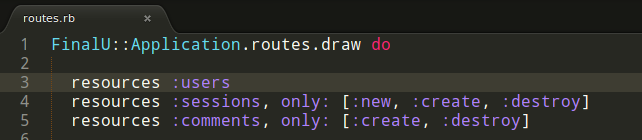
\includegraphics[width=1\textwidth]{rest}
        \end{center}
        \caption[REST - routes.rb]{config/routes.rb}
        \label{fig:rest}
      \end{figure}

      La figura \ref{fig:rest} muestra como se declara a \textbf{users} con 
      todas las acciones restful los cuales se listan en el cuadro \ref{tab:rest},  
      Rails también permite declarar solamente algunas acciones restful,
      como se ve el recurso \textbf{sessions} solamente tiene las acciones de \textbf{new}, \textbf{create} y \textbf{destroy}.\\
     

      \begin{table}[!hbp]
        \label{tab:rest}
        \begin{center}
          \begin{tabular}{ l l l  p{5cm} }
            \toprule
            \multicolumn{1}{c}{\textbf{HTTP}} & 
            \multicolumn{1}{c}{\textbf{URL}}  & 
            % \multicolumn{1}{c}{\textbf{C}}  & 
            \multicolumn{1}{c}{\textbf{ACCI\'ON}} &
            \multicolumn{1}{c}{\textbf{USADO PARA}}  \\
            \multicolumn{1}{c}{\textbf{request}} & & & \\

            \midrule
            GET     &   /users         &   index    & mostrar todos los usuarios\\ %\hline
            GET     &   /users/new     &   new      & genera un formulario HTML para crear un nuevo usuario \\
            POST    &   /users         &   create   & crea un nuevo usuario\\
            GET     &   /users/1       &   show     & muestra un usuario especifico\\
            GET     &   /users/1/edit  &   edit     & genera un formulario HTML para editar un usuario\\
            PUT     &   /users/1       &   update   & actualiza los datos de un usuario especifico\\
            DELETE  &   /users/1       &   destroy  & destruye un usuario\\
            \bottomrule
          \end{tabular}
          \caption[recursos REST]{las posibles rutas que se generan}
        \end{center}
      \end{table}

      Tal como se ve en el cuadro \ref{tab:rest}, Rails maneja los request HTTP de acuerdo con
      el tipo de llamada que se realice, este trabajo lo realiza el \textbf{router},    
      que reconoce las URLs y los despacha a una \textbf{acci\'on} del controlador,
      todo este proceso ya esta implementado en el nucleo de Rails por lo tanto  es autom\'atico y el programador
      no necesita mas configuraci\'on que la mostrada en la figura \ref{fig:rest}, 
      obedeciendo al principio de \emph{Convención sobre configuración}\\
 
      % % no son más que métodos dentro del \emph{user\_controller.rb} 
      % el cual 
      % es parte del controlador de la arquitectura MVC.\\

      % The Rails router recognizes URLs and dispatches them to a controller’s action. It can also generate paths and URLs, avoiding the need to hardcode strings in your views.

      Por ejemplo, si se genera una petición GET hacia la direcci\'on  
      \mbox{\emph{/usuarios/1}}  el servidor interpreta la dirección y responde 
      mostrando la información del usuario “1” ejecutando la acción 
      \textbf{show} del controlador usuarios y en cambio si se genera 
      una petición PUT a la misma direcci\'on \emph{/usuarios/1} el router 
      procesa la información y ejecuta la acción \textbf{update} del controlador 
      \textbf{usuarios} actualizando la información del usuario “1”. \\

      Esta convención de Rails ayuda a entender de mejor manera el flujo que tiene un recurso, 
      las URL son legibles y únicos para cada recurso. La implementación 
      de los recursos se hace de forma mas limpia y ordenada, situaciones que son 
      claves para el mantenimiento y la extensibilidad del sistema.


    % subsection rest (end)

    \subsection{MVC} % (fold)
    \label{sub:mvc}
      MVC (Modelo Vista  Controlador) es un patrón arquitectónico que separa 
      los datos de la aplicación en la interfaz del usuario y  la lógica del 
      negocio, en tres partes cada uno especializado para su tarea, la vista 
      maneja lo que es la interfaz del usuario, puede ser gráficamente o solo texto, 
      el controlador interpreta las entradas del teclado, mouse, o los cambios 
      de la vista de la mejor forma posible y finalmente el modelo maneja el comportamiento 
      de los datos de la aplicación.\cite{web7}
      Concepto que se desarrolló en 1979 por Trygve Reenskaug el cual da una 
      solución al problema de separar la lógica del negocio de la lógica de la presentación.\\ 
      % al final cada acción o concepto se desarrolla en un lugar determinado.\\
      % los objetivos/resultados/conclucion/facilidades
     
      Rails esta construido sobre el patr\'on MVC, esto significa que para cada
      pieza de código existe un lugar predeterminado y todas las piezas de código
      de la aplicacion interactuan de forma predeterminada. 
      \begin{description}
        \item[Modelo] Representa la informaci\'on o los datos y contiene 
        las reglas o métodos para manipular estos datos. En el caso de Rails, los
        modelos son usados principalmente para manejar la interacci\'on con las 
        tablas de la Base de Datos, en la que cada tabla corresponde a un modelo 
        en la aplicaci\'on, para nombrar a estos modelos existe una simple convenci\'on 
        que es la de nombrar  a la tabla en forma plural, mientras que el modelo 
        tiene el nombre en singular.
        El Modelo, en Rails es el principal encargado de manejar  la \emph{logica del negocio}.
        \item[Vista]  Representa la interfaz de la aplicaci\'on. En Rails las vistas 
        son archivos HTML con código Ruby embebido\footnote{ ERB (Embedded Ruby) } que realiza la tarea de representar 
        los datos. Las Vistas son las que generan los datos que son enviados al
        navegador web.%browser.
        \item[Controlador] Es el encargado de interactuar entre el modelo y la vista,
        procesando los datos enviados en el request del navegador web, 
        llamando a métodos del modelo para conseguir  \emph{informaci\'on} de la base de datos,
        posteriormente el controlador envia esta \emph{informaci\'on}  a la vista.

        El Controlador y la Vista son los los encargados de manejar  la \emph{l\'ogica de la presentaci\'on}.
      \end{description}

      % there’s a
      % place for each piece of code, and all the pieces of your application interact in a
      % standard way.

      \begin{figure}[!hbp]
        \begin{center}
          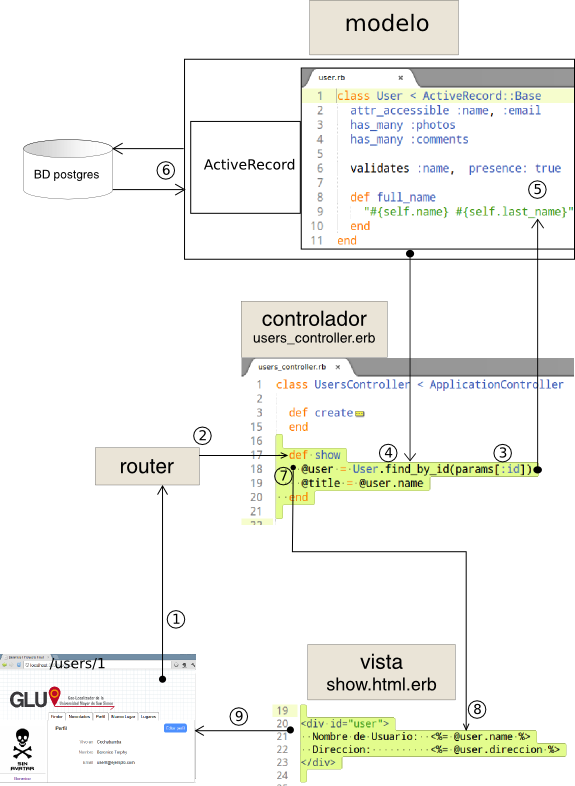
\includegraphics[width=1\textwidth]{mvc2}
        \end{center}
        \caption{Un diagrama detallado del patr\'on MVC en Rails}
        \label{fig:mvc}
      \end{figure}

      % \begin{figure}[!hdp]
      % \centering
      % \def\svgwidth{\columnwidth}
      % \input{mvc.pdf_tex}
      % \end{figure}


      Se puede apreciar el comportamiento de este patrón, en la figura \ref{fig:mvc}

      \begin{enumerate}
        \item se  generar un request ``\textbf{GET /users/1}'' desde el navegador web.
        \item este request primeramente es analizado por el \textbf{router}, que siguiendo el principio
        REST  lo direcciona a la acción \emph{show} del \textbf{controlador} \emph{users}.
        \item el controlador extrae el id del usuario de la llamada\footnote{ request} \textbf{GET /users/1}.
        \item la acción \emph{show} del controlador se encarga hacer la llamada al \textbf{modelo} ``User'',
        mediante el metodo \verb|find_by_id(1)|.
        \item el modelo ``User'', inicialmente valida o modifica los datos recibidos.
        \item el modelo ``User'', mediante el modulo ActiveRecord 
        extrae  la informaci\'on de la Base de datos.
        \item esta informaci\'on es almacenada en una
         \emph{instance variable}\footnote{los \emph{instance variable} son 
         variables especiales que empiezan con una ``@'' y están disponibles en la vista } \verb|@user|
        \item la vista ``show.html.erb''\footnote{ la extenci\'on \textbf{erb} 
        indica que la pagina HTML puede  tener contener código Ruby} incluye la variable \verb|@user| mediante los
        \emph{ERB output tag}(\verb|<%=  %>|)
        \item este template es procesado en el servidor, y renderizado como una 
        pagina HTML que es presentada en el navegador web.% mostrando la informacion
      \end{enumerate}


      % visitar la ruta que muestra la información de un usuario

      La capacidad de declarar una variable en el controlador y 
      que esta variable esté disponible en la vista, así como toda 
      la configuración que envuelve el comportamiento del patrón MVC 
      ya esta implementada y no es necesario escribir archivos de configuración, 
      El patr\'on MVC es la base de la aproximaci\'on RESTful de Rails, asi como  de las filosofías 
      \emph{DRY} y \emph{Convenci\'on sobre Configuraci\'on}, 
      %  y es el que hace 
      % posible 
      %  es parte   parte de la filosofía de Rails “convención sobre configuración”,
           en concluci\'on se pudo apreciar que       al usar esta arquitectura el código 
      se vuelve mas  ordenado, con el consiguiente resultado de ser un código 
      mucho mas limpio, legible y entendible. \\ %entendible\\


    % subsection mvc (end)

    \subsection{Mashup} % (fold)
    \label{sub:mashup}
      Mashup es una técnica en el desarrollo de aplicaciones web que consiste en 
      combinar datos de diferentes proveedores. Un mashup usa, uno o más servicios 
      y mezcla algunas características de estos servicios, los servicios generalmente 
      son datos que son distribuidos mediante las APIs\footnote{Application 
      Programming Interface, es el conjunto de funciones y procedimientos que se 
      ofrece para ser utilizado por otro software}. 

      Con la finalidad de ofrecer 
      estos datos de forma más fácil de entender y usar para el cliente.\\

      Los primeros mashups empezaron como experimentos con los web services que 
      ofrec\'ian las grandes empresas, por ejemplo uno de los primeros mashups mas
      importantes fue el de housingmaps\footnote{http://www.housingmaps.com/}  
      que combina los datos de Craigslist ( listas de casas, departamentos, etc, para rentar, vender ) 
      y Google Maps ( mapas a nivel global), en una aplicaci\'on que ofrece servicios y los 
      posiciona en un mapa. Desde entonces surgieron diferentes tipos y aproximaciones 
      dependiendo del tipo de datos y el servicio que se quiere ofrecer.\cite{web8}\\

      Se pueden apreciar diferentes implementaciones de mashups, los mashups 
      orientados al consumo y los mashups orientados a las empresas, básicamente 
      estos mashups de consumo se refieren a aplicaciones en las cuales los datos 
      obtenidos de diferentes fuentes son mezclados y presentados al cliente, 
      y los mashups empresariales o de negocios aparte de las fuentes de datos 
      externas, mezclan sus propios datos en el mashup ofreciendo una mejor experiencia del usuario.\\

      Uno de los componentes básicos de la Web 2.0 son los \textbf{datos},\cite{web5} 
      sobre los cuales se puede obtener un producto con valor agregado, 
      generalmente los datos están disponibles para que sean usados, pero
      dependiendo del tipo de ``datos'', obtenerlos y almacenarlos puede llegar a costar 
      tiempo o dinero o ambos, es por eso que los datos son ofrecidos con o sin 
      restricción dependiendo de las políticas de uso que tenga la empresa que ofrece los datos.\\

      El mashup implementado se podria catalogar como un mashup de negocio, ya que
      se esta integrando datos externos(Google Maps API) y datos internos(locaciones dentro del campus de la UMSS),
      inicialmente se almacenaron varias locaciones pero eventualmente estos datos
      se incrementaran mediante el uso que se le de por parte de los usuarios.\\

      % La figura \ref{fig:api_gm}, es necesario importar la
      % librería declarandola en la cabecera del documento HTML 

      %  para usar el y la figura \ref{fig:div_map} 
         
      Para usar el API de Google Maps es necesario importar la librería 
      declarandola en la cabecera del documento HTML, como se ve muestra en la 
      figura \ref{fig:api_gm}, para visualizar el mapa es 
      necesario declarar un elemento único (se recomienda un div con id de 
      preferencia ``map'' o similar) dentro del DOM de la página, figura 
      \ref{fig:div_map}, de esta forma se      logra visualizar el mapa 
      geográfico que ofrece Google, y su manejo es  mediante el lenguaje de 
      programación del lado      del cliente, \emph{javascript}, figura \ref{fig:umss_js}.\\

      Para el uso de los datos internos se hizo uso intensivo de la interfaz 
      REST de Rails, ya que se necesitaba desplegar en el mapa los lugares o locaciones
      de la UMSS, esto se debe a que la interfaz mashup se encuentra en el 
      lado del cliente(navegador Web) y la informaci\'on recopilada esta 
      almacenada en el servidor(Rails), entonces necesitaba extraer los datos del servidor y presentarlos al cliente, este procedimiento se lo puede demostrar con el uso del comando \verb|curl|, y con la informaci\'on obtenida se puede desplegar la locaci\'on en el mapa.\\

      \begin{center}
        \begin{verbatim}
          $ curl http://localhost:3000/places/23.json

          {
            "id": 23,
            "type": "caseta",
            "address": "",
            "lng": -66.1473755998898,
            "lat": -17.3938599682795,
            "name": "informaciones",
            "photos": [
              {
                "id": 28,
                "desc": "informaciones",
                "url": "photo/image/28/square_shin.jpg"
              }
            ]
          }
        \end{verbatim}
      \end{center}

      Como se ve en el ejemplo, el servidor responde mandando los datos en formato \textbf{json}\footnote{Notación de Objetos de JavaScript, es un formato ligero de intercambio de datos y  está basado en un subconjunto del Lenguaje de Programación JavaScript \cite{json}}, que al ser un metodo comun para enviar datos desde el servidor al cliente, es facil de implementar y de manipular, y se genera atraves de una plantilla 
      en la que se puede manipular los datos y presentarlos de la mejor forma posible. Por ejemplo para mostrar los lugares se escribio la siguiente plantilla.

      \begin{center}
        \begin{verbatim}
          # views/places/show.json.rabl

          object  @place
          attributes :id, :name, :desc, :address

          node(:type) { |place| place.type_place.name }
          node(:lng)  { |place| place.coord_geographic.x }
          node(:lat)  { |place| place.coord_geographic.y }

          child :photos do 
            attributes :id, :desc
            node(:url) { |photo| photo.image.url(:square) }
          end
        \end{verbatim}
      \end{center}


      De esta forma se pueden ofrecer los datos internos para que otras aplicaciones la puedan usar. Es lo que se denominaria \emph{REST Web Services}\\


      En la aplicación desarrollada se necesitaba el uso de mapas para que el 
      despliegue de información sea de forma más interactiva y de fácil uso, 
      los datos geográficos públicos generalmente están disponibles para ser 
      usados pero para su uso se necesitaba que esté representado de forma gráfica 
      en la pantalla de la computadora, este trabajo lo llevan a cabo empresas 
      las cuales generalmente cobran por el uso de los mapas, se puede  apreciar 
      que se están obteniendo datos en forma de mapas a través del API de Google Maps, 
      Google permite usar sus datos con restricciones dependiendo de la cantidad 
      de llamadas que se haga a su API por la aplicación que la usa.\\

      El gran beneficio de usar los datos de Google Maps en un mashup es que nos 
      permite desplegar información que de otra forma costaría mucho tiempo y dinero para implementar.\\


      \begin{figure}[!hbp]
        \begin{center}
          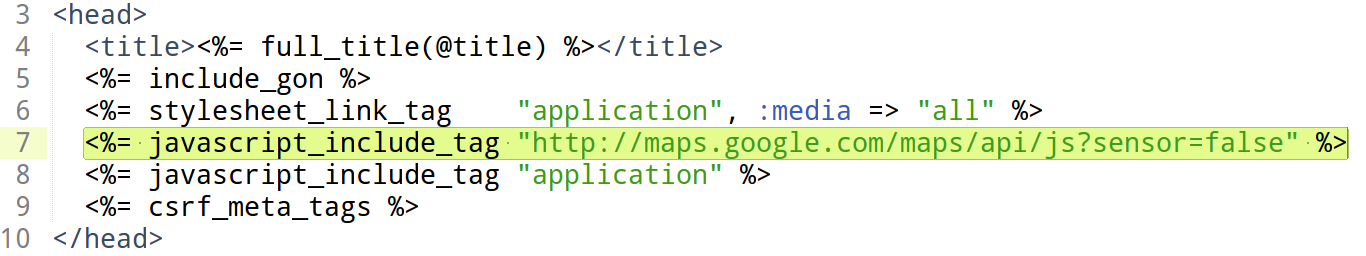
\includegraphics[width=1\textwidth]{api_gms}
        \end{center}
        \caption[API de Google Maps declarado]{Se importa el API de Google Maps declarando en  <head>  ~del documento}
        \label{fig:api_gm}

        % \vspace{4em}

        \begin{center}
          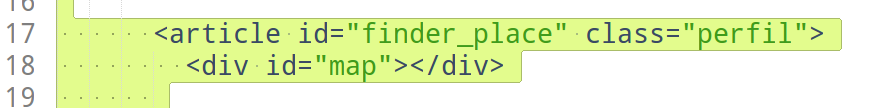
\includegraphics[width=1\textwidth]{div_map}
        \end{center}
        \caption[Div con id map para el Mapa]{El mapa se visualiza dentro de la etiqueta div con id map}
        \label{fig:div_map}

        % \vspace{4em}

        \begin{center}
          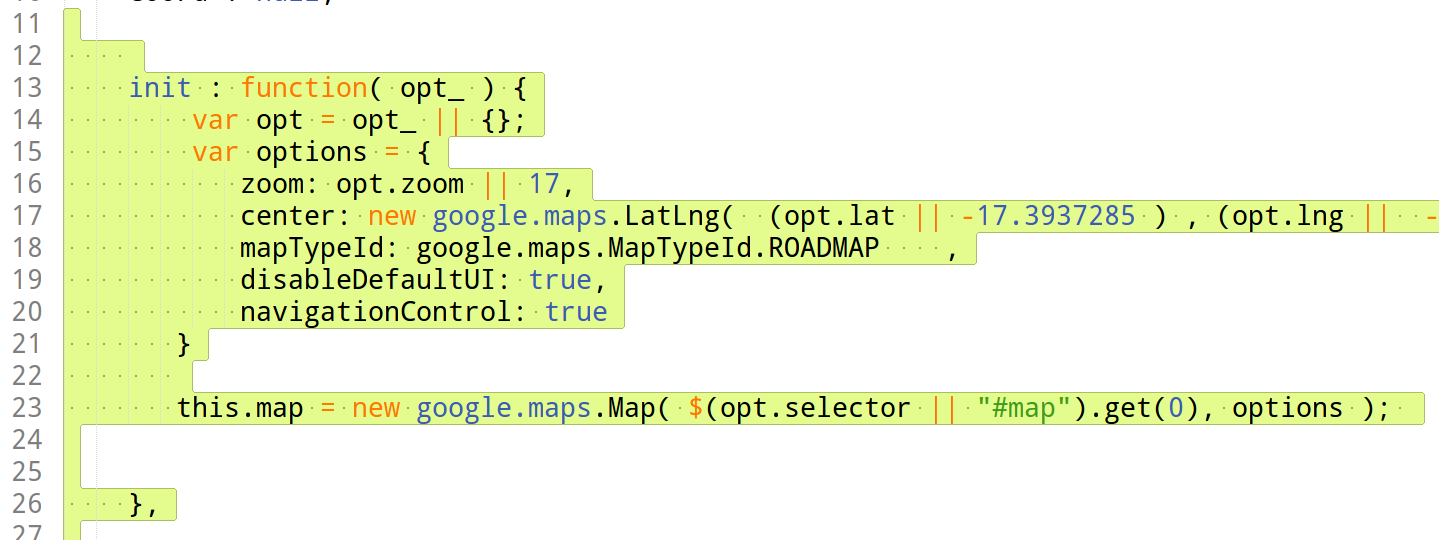
\includegraphics[width=1\textwidth]{umss_init}
        \end{center}
        \caption[UMSS javascript]{Se captura el div map del documento y se inicializa el mapa mediante el lenguaje javascript}
        \label{fig:umss_js}
      \end{figure}
      
        % \vspace{4em}
      % \begin{figure}[!hbp]
      %   \begin{center}
      %     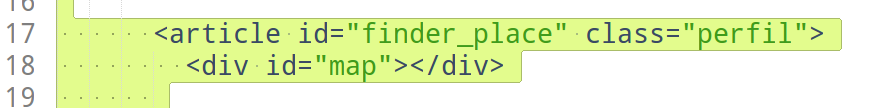
\includegraphics[width=1\textwidth]{div_map}
      %   \end{center}
      %   \caption[Div con id map para el Mapa]{El mapa se visualiza dentro de la etiqueta div con id map}
      %   \label{fig:div_map}
      % \end{figure}


      % \begin{figure}[!hbp]
      %   \begin{center}
      %     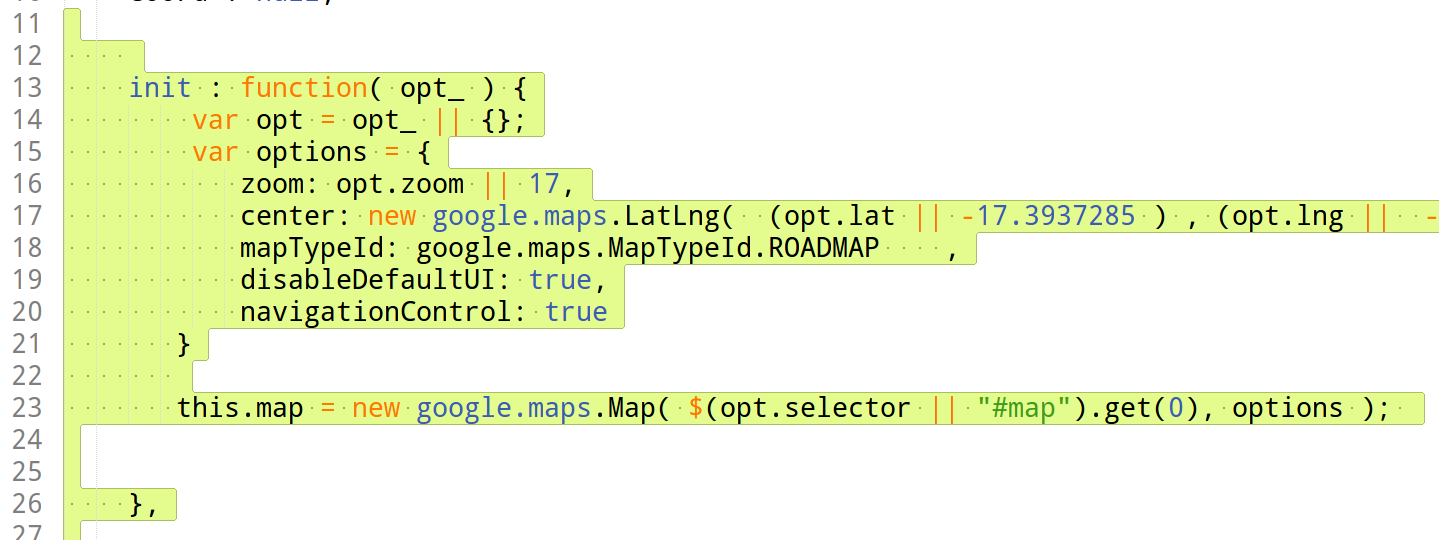
\includegraphics[width=1\textwidth]{umss_init}
      %   \end{center}
      %   \caption[UMSS javascript]{Se captura el div map del documento y se inicializa el mapa mediante el lenguaje javascript}
      %   \label{fig:umss_js}
      % \end{figure}

    % subsection mashup (end)
  % section patrones_web20 (end)

  \section{Concluci\'on} % (fold)
  \label{sec:conclucion}
    Los patrones no son entidades separadas, como ya se vio todos los patrones web2.0 
    se integran y trabajan de manera conjunta, no se podría implementar software que solo 
    implemente algun patr\'on.
    
    Los patrones empiezan como soluciones a algun problema de dise\~no y descritas en concepto, 
    gracias a que los problemas y experiencias que tuvieron los programas que lograron pasar de la
    Web Estatica  y los que nacieron en la Web2.0 están documentados y analizados,
    después depende de los desarrolladores el implementarlas de la mejor forma posible.\\

    Rails se dise\~no, para que trabaje sobre las ultimas tecnolog\'ias disponibles, para poder desarrollar 
    software que se pueda catalogar como ``\emph{Aplicacion Web2.0}'', pero al final que una aplicaci\'on
    obtenga esta etiqueta esta dada por m\'ultiples factores, tales que pueden ser,
    la capacidad de entender la web como un algo que evoluciona con el tiempo, e
    implementar software que pueda utilizar todos los avances tecnol\'ogicos en favor
    de mejorar la experiencia del usuario, siempre apoyados por la interacci\'on
    que supone el intercambio y flujo de ideas de la comunidad de usuarios que usan
    la aplicaci\'on.\\  
    % ser mejorado, actualizado, analizado por sus usuarios.  
    
 
    % por eso tiene gran importancia estudiar los  patrones, para obtener una idea clara de 

  % section conclucion (end)
% chapter ruby_on_rails_y_patrones_web_2_0 (end)


  
  \chapter{Geolocalizaci\'on} % (fold)
\label{cha:geolocalizacion}
  La Geolocalizaci\'on o Georreferenciación es un termino bastante nuevo, de hecho no aparece en el diccionario de la Real Academia Espa\~nola, no obstante se lo puede definir como:
  \begin{quote}
    El posicionamiento en el que se define la localización de un objeto espacial (representado mediante un punto, vector, área, volumen) en un sistema de coordenadas y datum determinado. Este proceso es utilizado frecuentemente en los Sistemas de Información Geográfica.
  \end{quote}

  % Para entender esta definición se necesita explicar algunos terminos     

  La Georreferenciación era usada bastante en el ambito científico, y se necesitaba de instrumental y personal bastante cualificado para su manejo, pero en la actualidad la cantidad de dispositivos con capacidad para geolocalizar un objeto sobre la tierra es bastante comun, de hecho todos los smartphones actuales (celulares con Android, Iphones) traen integrados receptores GPS (Global Posicion System),  y sumados a la exploci\'on de aplicaciones  que integran mapas con localizaci\'on (mashups), ya que se puede tener una base de datos con informaci\'on muy importante pero al final  los datos son cifras, descripciones, etc. y para tomar decisiones se hace muy difícil el interpretar estos datos, aca viene en nuestra ayuda los SIG (Sistemas de Informaci\'on Geografica).\\

  Actualmente existe una explosi\'on de aplicaciones, donde empresas, particulares y hasta donde organismos gubernamentales est\'an haciendo uso de estas tecnologías.
  Y las posibilidades son diversas, por ejemplo, se se quisiera planificar la construcci\'on de un colegio se podria integrar los datos del censo con un mapa, identificando los sectores con mayor porcentaje de ni\~nos y localizando los sectores mas propicios para realizar la construcción del inmueble. En el caso de una catástrofe natural, el tener las rutas de evacuaci\'on geolocalizadas y disponibles en un mapa de manera eficiente,  ayudaria en la evaciaci\'on de las personas del lugar.\\ 

   
  \section{Definiciones} % (fold)
  \label{sec:definiciones}
  
    En la aplicaci\'on desarrollada se requería trabajar con datos espaciales, y para ello es necesario entender algunos conceptos envueltos en el manejo de la informaci\'on geografica.

    \begin{description}
      \item[Coordenada] Es una secuencia de n-numer\'os que designa la posici\'on de un punto en un espacio n-dimensional. \\
      \item[Sistema de coordenadas] Un sistema de coordenadas es  un conjunto de reglas matemáticas que especifican como las coordenadas son asignadas  a cada  punto.
      \item[Punto] Es  la representaci\'on de una posici\'on, topol\'ogicamente 0-dimensional (no tiene volumen, area, longitud o cualquier otra unidad multi-dimensional).
    \end{description}

    % \subsection{Coordenada} % (fold)
    % \label{sub:coordenada}
    %   Es una secuencia de n-numer\'os que designa la posici\'on de un punto en un espacio n-dimensional. \\
    %   % one of a sequence of n-numbers designating the position of a point (4.17) in n-dimensional space
    %   % NOTA: En un 
    %   % NOTE In a coordinate reference system, the numbers shall be qualified by units.

    % % subsection coordenada (end)

    % \subsection{Sistema de coordenadas} % (fold)
    % \label{sub:sistema_de_coordenadas}
    %   Un sistema de coordenadas es  un conjunto de reglas matemáticas que especifican como las coordenadas son asignadas  a cada  punto.
    %   % set of mathematical rules for specifying how coordinates (4.3) are to be assigned to each point (4.17)

    % % subsubsection sistema_de_coordenadas (end)
    % \subsection{Punto} % (fold)
    % \label{sub:punto}
    %   Es  la representaci\'on de una posici\'on, topol\'ogicamente 0-dimensional (no tiene volumen, area, longitud o cualquier otra unidad multi-dimensional).  
    %   % topological 0-dimensional geometric primitive (4.15), representing a position
    % % subsection punto (end)

    Estas definiciones estan desarrolladas en la especificaci\'on \textbf{Simple Feature Access}, la cual es mantenida por la OGC (Open Geospatial Consortium). Esta especificaci\'on define el conjunto de tipos de datos (puntos, linia, poligono, etc) y las operaciones o metodos necesarios para manejar estos datos.
    
  % section definiciones (end)
  \section{Sistema de Coordenadas para datos Geográficos} % (fold)
  \label{sec:sistema_de_coordenadas_para_datos_geograficos}
    Se podria pensar en un sistema de coordenadas como la forma de dar sentido a un \emph{par de coordenadas}, por ejemplo cuando se ve una locaci\'on ``\verb|POINT(-66.1457475 -17.3937285)|'', como se interpretan estos n\'umeros?.
    Podria ser la latitud y longitud del campus de la UMSS, o podria ser un sistema de a\~nos luz desde alguna estrella en el Universo.
    El sistema de coordenadas es lo que diferencia estos casos.\\


    Una aplicaci\'on que maneja datos geograficos, generalmente trabaja con sistemas de coordenadas relacionadas con la superficie terrestre, conocidas como coordenadas espaciales (coordenadas globales), que permiten representar la tierra en 3-Dimensiones (3D), ya que esta es una Esfera (elipsoide oblato), o en una representacion de la superficie terrestre en 2-Dimensiones (2D), se pueden nombrar los siguientes:

    \subsection{Coordenadas geocéntricas (X,Y,Z)} % (fold)
      \label{sub:coordenadas_geocentricas}
        También conocido como Coordenadas Cartesianas 3D, Este sistema tiene como origen el centro de la Tierra, con el eje X y el eje Y en el plano del ecuador. El eje X pasa a través del meridiano de Greenwich, y el eje Z  coincide con el eje de rotación de la Tierra.

        \begin{figure}[!hbp]
          \begin{center}
            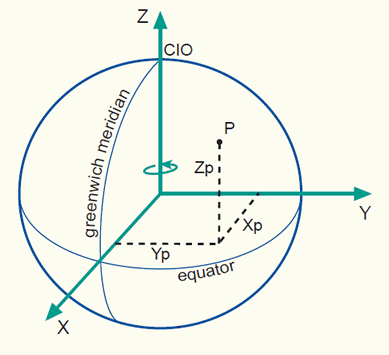
\includegraphics[width=0.7\textwidth]{coord_geocentric}
          \end{center}
          \caption[Sistema de coordenadas Geocentricas ]{Sistema de coordenadas Geocentricas, en la figura se muestra la posici\'on del punto P}
          \label{fig:coord_geocentric}
        \end{figure}

        Este Sistema de coordenadas no es muy usado en la representacion de datos.
        % , pero aveces se lo requiere para analisis de algoritmos y geometria computacional.
      % subsection coordenadas_geocentricas (end)  

      \subsection{Coordenadas Geograficas} % (fold)
      \label{sub:coordenadas_geograficas}
        Sistema de coordenadas Geográfico, utiliza las coordenadas angulares latitud  (phi o ${\phi}$) y longitud (lambda o ${\lambda}$). Este sistema de coordenadas se expresa en grados, se lo puede representar con la forma \emph{grados:minutos:segundos }\verb|(17° 23' 37.4226" S, 66° 8' 44.691" W)|, o de la forma mas comun \emph{grados decimales} \verb|(-66.1457475 S, -17.3937285 W)|.\\

        El sistema de coordenadas  mas amplimente usado, el que usan por defecto los sistemas GPS, es conocido como ``WGS 84'', y la mayoria de las aplicaciones que manejan mapas.\\

        \begin{figure}[!hbp]
          \begin{center}
            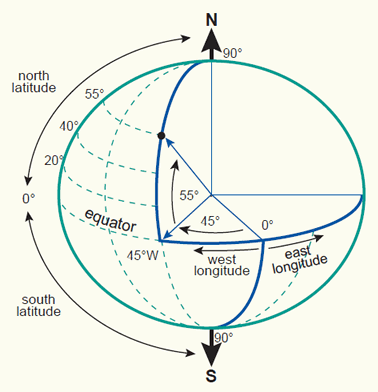
\includegraphics[width=0.7\textwidth]{coord_geographic}
          \end{center}
          \caption[Sistema de coordenadas Geográficos]{Sistema de coordenadas Geográficos, Es el sistema que maneja los mas amplimanete conocidos ``latitud y longitud''} 
          \label{fig:coord_geographic}
        \end{figure}   

      % subsection coordenadas_geograficas (end)

      \subsection{Coordenadas Proyectadas} % (fold)
      \label{sub:coordenadas_proyectadas}
        Un sistema de coordenadas proyectadas es una representación plana y bidimensional de la  tierra. Se basa en un sistema de coordenadas geográficas esf\'ericas, pero utiliza unidades de medida lineales para las coordenadas, de forma que los cálculos de distancia y área se pueden realizar en términos de esas mismas unidades.\cite{projected_ibm} \\

        Un sistema de coordenadas proyectadas requiere tomar la superficie esferica de la tierra y ``aplanarla'', este procedimiento se lo realiza con la finalidad de tener un mapa representable en una hoja de papel asi como en la pantalla de la computadora. Sin embargo este procedimiento introduce diversos tipos de distorci\'on por lo que existen diferentes clases de proyeciones que varian segun la region que se quiere representar de la Tierra.\\

        La proyecci\'on que usa Google Maps es la \textbf{Mercator Projection}, esta proyecci\'on esta dise\~nada para presevar los ángulos y las formas de las linias en forma recta, pero distorciona los tama\~nos y las distancias mientras mas lejos se encuentran de la linia del Ecuador. Esta proyecci\'on se puede apreciar en la figura \ref{fig:mercator_proyection}

        \begin{figure}[!hbp]
          \begin{center}
            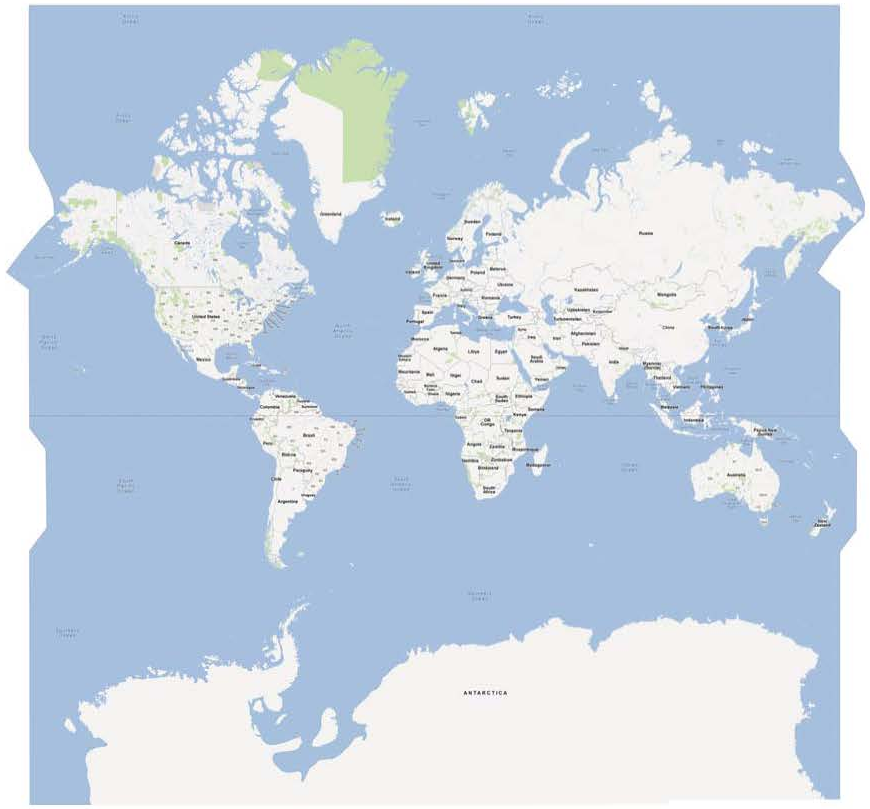
\includegraphics[width=0.6\textwidth]{mercator_proyection}
          \end{center}
          \caption[Sistema de coordenadas Proyectadas]{Google Maps usa la Proyección de Mercator para mostrar su mapa} 
          \label{fig:mercator_proyection}
        \end{figure}

        Tal como se puede apreciar en la figura \ref{fig:mercator_proyection}, la distorcion de esta proyecci\'on se hace evidente si se observa la zona de Groenlandia ya que pareceria tan grande como Africa o America del Sur, cosa que no es, ya que Groenlandia es casi 14 veces mas peque\~no que Africa. A pesar de esta distorci\'on tan marcada, la \textbf{Proyección de Mercator} es una de las mas usadas.
         % de hecho Google Maps usa esta proyecci\'on.
      % subsection coordenadas_proyectadas (end)
      \subsection{Que se uso en la Aplicaci\'on} % (fold)
      \label{sec:que_se_uso_en_la_aplicacion}
        Es importante entender las diferencias entre los distintos tipos de sistemas de coordenadas porque computacionalmente realizar operaciones sobre los sistemas de coordenadas tiene un costo.        
        Si se usara el sistema de coordenadas geográfico (WSG84) este es el más apropiado si se necesitaria usar grandes extensiones de la superficie terrestre, que al ser una estructura elipsoidal el costo computacional para realizar las operaciones matemáticas de calcular distancias, intersecciones, etc. es más elevado. En cambio el uso de un sistema de coordenadas proyectado (Mercator Projection) tiene un costo computacional más bajo, ya que se estaría trabajando con un sistema geométrico.\\

        % Por otro lado, 
        También hay tomar en cuenta la base de datos, ya que será esta la que se encargara de manejar los datos espaciales. Al estar usando PostGIS, se puede ver que en su documentacion\footnote{ http://postgis.org/documentation/manual-1.5/ch04.html} que claramente exorta el uso de un sistema geometrico sobre el uso de un sistema geografico si  se va trabajar con datos que cubran una peque\~na area geografica. Tomando en cuenta esta recomendaci\'on y el tama\~no del área de estudio (campus UMSS), se procedió a implementar en la base de datos el uso de la proyecci\'on Mercator. Se va usar Mercator sobre las otras proyecciones porque aparte de las ventajas que se mencionaron con anterioridad, Google Maps usa esta proyecci\'on y ya que se usara este mapa lo más correcto es trabajar con la misma proyecci\'on.  
       

        % Como 
        % PostGIS maneja dos tipos de datos, geograficos y geometricos

      % section que_se_uso_en_la_aplicacion (end)
  % section sistema_de_coordenadas_para_datos_geograficos (end)

  \section{Implementaci\'on} % (fold)
  \label{sec:Implementacion}
    Al implementar una aplicaci\'on con Rails, no se maneja la base de datos con ordenes SQL  puro. La base de datos se la maneja atraves de un ORM (ActiveRecord). 
    Para llevar a cabo esta tarea es necesario escribir una \emph{migraci\'on}, el cual es un metodo que Rails interpreta y lo traduce a ordenes SQL.\\
    \begin{center}
      \begin{verbatim}
        class CreatePlaces < ActiveRecord::Migration
          def change
            create_table :places do |t|
              t.string :name
              t.point :coord, :srid => 3785 
            end
          end
        end
      \end{verbatim}
    \end{center}
    Esta \emph{migraci\'on} cre\'o la tabla \textbf{places} con los atributos \textbf{name} y \emph{coord}, el atributo \textbf{name} es del tipo string que en PostgreSQL se traducir\'ia en una columna de tipo \emph{VARCHAR(255)}, y el atributo \textbf{coord} de tipo point con un srid\footnote{ Spatial Reference System Identifier, El SRID corresponde a un sistema de referencia espacial basado en el elipsoide concreto usado para la creación de mapas de tierra plana o de tierra redonda.\cite{msdn_srid} } 3785,     el SRID  es la llave primaria de la tabla \emph{spatial\_ref\_sys} que se crea cuando se inicializa una base de datos espacial, esta tabla provee la informaci\'on necesaria para interpretar y convertir correctamente todas las coordenadas existentes, adem\'as permite definir alg\'un tipo de sistema de coordenadas si no existe en esta tabla, el SRID 3785 esta definida en la tabla \emph{spatial\_ref\_sys}  como ``Popular Visualisation CRS / Mercator'', Rails interpreta el tipo point y crea una columna de tipo \emph{geometry}, definida por PostGIS.\\

    El anterior código escrito en Rails se traduciria en SQL de la siguiente forma: 
    \begin{center}
      \begin{verbatim}
        CREATE TABLE places (
          id    INTEGER       PRIMARY KEY,
          name  VARCHAR(255)
        );
        SELECT AddGeometryColumn(
                  'places', -- 'nombre_tabla'
                  'coord',  -- 'nombre_columna'
                  3785,     -- srid
                  'POINT',  -- 'tipo'
                  3         -- dimension
               );
      \end{verbatim}
    \end{center}
    Al usar un framework como Rails, se tiene como ventaja que existen herramientas creadas, comprobadas y avaladas por una gran catidad de usuarios, en este caso se preciso de herramientas que ayuden en el  manejo de informaci\'on geogr\'afica, la gema \textbf{RGeo} es la que maneja  la correcta manipulaci\'on de estos datos. 


  % section Implementacion (end)

  \section{Concluci\'on} % (fold)
  \label{sec:geo_conclucion}
    Los Mapa son herramientas muy útiles a la hora de desplegar información pero realizar el mapa, crear las fórmulas matemáticas con las cuales se trabajará, determinar cómo se usarán estas fórmulas para una representación adecuada de la superficie terrestre, es una tarea muy compleja. Como programador la tarea más complicada fue determinar el tipo de mapa y el sistema de coordenadas más adecuado al trabajo.\\

    Los términos de longitud y latitud son en un inicio, más fácilmente comprendidos que un sistema proyectado, pero no se puede tomar a la ligera una correcta comprensión del uso de los sistemas de coordenadas en una base de datos espacial, un mal uso de estos conceptos puede generar errores a la hora de manejar datos  espaciales o en el resultado de operaciones sobre estos  datos.



    % Maps are deceivingly simple tools, and cartography a surprisingly complex discipline. While the most trouble many of us will have with a map is figuring out how to fold it, this simplicity belies great sophistication that has been developed over the years. 
  % section geo_conclucion (end)


  % \begin{description}
  %   % \item[SIG] Un Sistema de Informaci\'on Geografica es una manera de visualizar c\'omo es y que est\'a ocurriendo en algun lugar. La posibilidad de incorporar coordenadas con presici\'on.

  %   % A GIS is a colletion of software, normaly manipulatedby its user through a single interface, and designed to perform a wide range of operations on geographic data.  
  %   % Research  Methods in Geography
  %   % Basil Gomez and John Paul Jones III.
  %   % ISBN 978-1-4051-0710-5

  %   \item[Datum] 
  %   \item[] 
  %   \item[] 
  % \end{description}

  % procesar
  % Se tien
  % , Sistema de Posicionamiento Global por sus siglas en espa\~nol
% chapter geolocalizacion (end)

   
  % \chapter{Ruta Optima} % (fold)
\label{cha:ruta_optima}
  

  Si se quiere ir de un punto a otro el mejor camino siempre es el mas optimo, pero como se define que un camino sea óptimo, si se va en coche hay que tomar en cuenta la dirección de las calles, los cruces, etc. si se va a pie hay que ver las características del terreno, caminos cortados, distancias, etc. 


  Si se analiza el terreno que se va a cubrir con la aplicación (el campus de la UMSS), se tiene que el  camino optimo es siempre el más corto o de menor longitud. 

  La resolución de este problema es la se analizará en este capítulo.

  \section{Grafos} % (fold)
  \label{sec:teoria_grafos}
  
    El problema es encontrar la ruta más corta de un punto a otro punto, en donde los puntos están interconectados por una red de caminos. El problema descrito se lo puede resolver/describir como un caso espec\'ifico de la teoría de grafos.


    \subsection{Definiciones} % (fold)
    \label{sub:grafos_definiciones}
      Primeramente se aclarar\'an alguno términos usados en la teoría de grafos.\\

      % El grafo que es la reprentacion 

      % \begin{description}
      %   \item[Grafo] Un grafo G consiste en un conjunto  vértices V y un conjunto de aristas A, y se lo escribe como G(V,E).
      %   \item[Vertice] 
      % \end{description}
      
      Un \textbf{grafo} $G$ consiste en un conjunto de vértices $V$ y un conjunto de aristas $A$, y se lo representa con $G(V,A)$.\\ 

      El \textbf{vértice} \emph{v} es adyacente a \emph{u}, o a un vecino de \emph{u}, si y sólo si $(u,v) \in A$. Por lo tanto, en un grafo no dirigido, dado una arista $(u,v)$, $v$ es adyacente de $u$, y simétricamente \emph{u} es adyacente de \emph{v}. 
      Los vértices también son llamados nodos. \\

      Cada \textbf{arista} o arco es representada por un par de elementos $(u,v)$, donde los elementos $u,v \in V$, son los nodos que une la arista.
      En un grafo no dirigido el par de vértices que representan la arista no tiene orden, por lo tanto la arista $(u,v)$ y $(v,u)$ representa la misma arista. En cambio en un grafo dirigido la arista $(u,v)$ y $(v,u)$ representan dos diferentes aristas. También se puede anotar un tercer componente, llamado peso o costo, en ese caso estaríamos hablando de un \emph{grafo ponderado}.\\
      % Para fines prácticos, no  consideraremos las aristas de la forma (u,u)

      En un grafo no dirigido $G$, dos vértices $u$ y $v$ se dice que están conectados si hay un camino en $G$ de $u$ a $v$ (y como $G$ no es dirigido, también hay un camino de $v$ a $u$). Un grafo  se denomina completo si para todos los pares $u,v \in V$ existe una arista $(u,v) \in A$.\\

      Un camino en un grafo es una secuencia de nodos $v_{1}$, $v_{2}$, ... , $v_n$ tal que $(v_{1}, v_{2}), (v_{2}, v_{3}), ... , (v_{n-1}, v_n)$ son aristas. 
    % \end{description}
    % subsection grafos_definiciones (end)
    \subsection{Representacion de un Grafo} % (fold)
    \label{sub:representacion_de_un_grafo}
      Existen diversas formas de representar un grafo sea dirigido o no-dirigido, pero entre las mas usadas están la matriz de adyacencias y la lista de adyacencias.
      \subsubsection{Matriz de adyacencias de un Grafo} % (fold)
      \label{ssub:matriz_de_adyacencias_de_un_grafo}  
        Sea $G = (V,A)$ un grafo de \emph{n} vértices. La matriz de adyacencias $M$  para $G$ es una matriz $M_{nxn}$ de valores booleanos, donde $M(i,j)$ es verdad si y sólo si existe un arco desde el nodo \emph{i} al nodo \emph{j}.

        \begin{displaymath}
          M(i,j) = \left\{ 
          \begin{array}{ l l }
            1, & \textrm{si existe la arista } (i,j) \\
            0, & \textrm{en caso contrario}
          \end{array} \right.
        \end{displaymath}


        Las filas y las columnas de la matriz representan los nodos del grafo.
        Cuando el grafo no es dirigido la matriz de adyacencias es simétrica.
        % El cuadro \ref{tab:matriz} representa la matriz de adyacencias de la figura \ref{fig:grafo_ponderado} representa 
        La matriz de adyacencias, que se puede observar en el cuadro \ref{tab:matriz}, es la  misma matriz de la relación $A$ de $V$ en $V$ porque indica cuales v\'ertices están relacionados (unidos por una arista)


        \begin{figure}[!ht]
          \begin{center}

            \begin{tikzpicture}[->,>=stealth',shorten >=1pt,auto,node distance=3cm,
                    main node/.style={circle,draw,font=\sffamily\Large\bfseries}]
                    
              \node[main node] (1) {a};
              \node[main node] (2) [below right  of=1] {b};
              \node[main node] (3) [above right of=2] {c};
              \node[main node] (4) [below left of=2] {d};
              \node[main node] (5) [right of=2] {e};
              % \node[main node] (6) [right of=5] {f};
              % \node[main node] (7) [above right of=6] {g};
              % \node[main node] (4) [below right of=1] {d};

              \path[every node/.style={font=\sffamily\small}]
                (1) edge node [auto] {3} (2)
                    edge node[left] {5} (4)
                (2) edge node[left] {8} (3)
                    edge node[right] {4} (4)
                    edge node[auto] {3} (5)
                (3) edge node[left] {7} (5)
                (4) edge node[below] {14} (5);
                
            \end{tikzpicture}

          \end{center}
          \caption{Grafo ponderado no-dirigido}
          \label{fig:grafo_ponderado}
        \end{figure}

        \begin{table}[!ht]
          \label{tab:matriz}
          \begin{center}
            \begin{displaymath}
              M(i,j) =
              \bordermatrix{ ~ & a & b & c & d & e \cr
                             a & 0 & 3 & 0 & 5 & 0 \cr
                             b & 3 & 0 & 8 & 4 & 3 \cr
                             c & 0 & 8 & 0 & 0 & 7 \cr
                             d & 5 & 4 & 0 & 0 & 14\cr
                             e & 0 & 3 & 7 & 14& 0  }
            \end{displaymath}
            \caption{Matriz de adyacencias del grafo de la figura  \ref{fig:grafo_ponderado}}
          \end{center}
        \end{table}


      % subsubsection matriz_de_adyacencias_de_un_grafo (end)
      
    % subsection representacion_de_un_grafo (end)
    \subsection{Ruta mas corta} % (fold)
    \label{sub:ruta_mas_corta}
      Dados los vértices $v_{i}$ y $v_{j}$ de un grafo G = (V,A) se llama trayectoria mínima o camino minimo  de \(v_i\) a \(v_j\) al numero de aristas del camino de longitud mínima que va desde $v_i$ a $v_j$ y se representa por $d(v_i, v_j)$.

      Cuando en el grafo no exista un camino de $v_i$ a $v_j$ se dice que el camino minimo es $d(v_i, v_j) = oo$ \\

      Para determinar el camino mínimo que va desde un único vértice a cualquier otro vértice se puede usar el algoritmo de Dijkstra. 
      


      \subsubsection{Algoritmo de Dijkstra} % (fold)
      \label{sub:algoritmo_de_dijkstra}
      El algoritmo de  Dijkstra fue descrito en 1959 por Edsger Dijkstra, y permite encontrar la trayectoria más corta entre dos nodos específicos, cuando los valores de los arcos son todos positivos\\

      El algoritmo asigna un etiqueta a cada nodo en el grafo. Esta etiqueta es la distancia que hay desde el nodo s escogido como origen a lo largo de la trayectoria más corta encontrada, hasta el nodo que se está etiquetando.\\

      La etiqueta de cada nodo puede estar en 2 estados:

      \begin{itemize}
        \item[a.] Puede ser permanente: en este caso la distancia encontrada es a lo largo de la trayectoria más corta de todas las encontradas.
        \item[b.] Puede ser temporal: cuando hay incertidumbre de que la trayectoria encontrada sea la más corta de todas.
      \end{itemize}

      A medida que el método trabaja se cambian gradualmente las etiquetas temporales por etiquetas permanentes. Al comienzo se tiene un conjunto de nodos con etiquetas temporales y el objetivo es hacer que esas etiquetas disminuyan, encontrando trayectorias a esos nodos usando trayectorias a nodos etiquetados permanentemente. Cuando esto se ha logrado, se selecciona el nodo con la etiqueta temporal más pequeña y esta etiqueta se convierte en permanente. El proceso se repite hasta que al nodo terminal t se le haya asignado una etiqueta permanente, pero esto puede ocurrir eventualmente, ya que cada vez que el algoritmo es usado, una de las etiquetas es omitida y así el número de nodos con etiquetas temporales decrece a cero. \cite{teoria_grafos} \\

      
      % subsection algoritmo_de_dijkstra (end)
    % subsection ruta_mas_corta (end)
  % section teoria_grafos (end)
  
  \section{Conclusion} % (fold)
  \label{sec:ruta_conclusion}

    Existen numerosas soluciones para encontrar la ruta óptima, donde se toman en cuenta diferentes variables y heurísticas, en el que  cada algoritmo presenta ventajas respecto a las demás.
    La teoría de grafos  es un tema extenso y para fines prácticos 
    solo se explicó el algoritmo de Dijkstra por ser el que se esta usando en la aplicación desarrollada.\\
    
    El algoritmo de Dijkstra puede ser una de las soluciones más sencillas y que requiere muchos más cálculos que las demás pero el grafo implementado al no ser extenso, no existe una razón de mucho peso para buscar otra solución más eficiente en el manejo de recursos.

  % section ruta_conclusion (end)
% chapter ruta_optima (end)


  % Algoritmos de busqueda de caminos - ruta corta

  % Como determino que tipo de grafo tengo


  % % \section{La Red} % (fold)
  % % \label{sec:la_red}
  
  % % % section la_red (end)

  % \section{Algoritmo} % (fold)
  % \label{sec:algoritmo}
  
  % % section algoritmo (end)

  % \section{Algoritmo de Dijkstra} % (fold)
  % \label{sec:algoritmo_de_dijkstra}
  
  % % section algoritmo_de_dijkstra (end)
  
  % % Por lo tanto se implementó un grafo no dirigido (sin dirección), el cual se analizará en este capítulo.


  % Un problema de este tipo es represetable como un proble de teoria de grafos.


  % Cuando se tiene que encontrar un camino o ruta optima entre 2 puntos, se tienen que tomar en cuenta varios puntos


  % El problema de encontrar una ruta optima entre 2 puntos se lo puede resolver/representar como problema de grafos


  % Caminos mínimos en grafos

  % Solución voraz: Algoritmo de Dijkstra

  % para grafos dirigidos (la extensión a no dirigidos es inmediata)
  % genera uno a uno los caminos de un nodo v al resto por orden creciente de longitud
  % usa un conjunto de vértices donde, a cada paso, se guardan los nodos para los que ya se sabe el camino mínimo
  % devuelve un vector indexado por vértices: en cada posición w se guarda el coste del camino mínimo que conecta v con w
  % cada vez que se incorpora un nodo a la solución se comprueba si los caminos todavía no definitivos se pueden acortar pasando por él
  % se supone que el camino mínimo de un nodo a sí mismo tiene coste nulo
  % un valor en la posición w del vector indica que no hay ningún camino desde v a w
  % E.W. Dijkstra:
  % “A note on two problems in connexion with graphs”,
  % Numerical Mathematica, 1, pp. 269-271, 1959.

  \chapter{Descripci\'on de la implentaci\'on} % (fold)
\label{cha:descripcion_de_la_implentacion}


  
  % la aplicacion se realizo sobre ruby on rails 
  La aplicacion a desarrollar requeria de implementar un sistema de geolocalizaion, para tal motivo primeramente se procedio a generar un mapa de rutas sobre la cual escoger las herramientas mas apropiadas para la realizacion de la aplicacion.

  \section{Generaci\'on de las rutas} % (fold)
  \label{sec:generacion_de_las_rutas}
    Se procedio a trazar un mapa de rutas del campus de la Universidad Mayor de San Simon, para tal efecto se necesito de un GPS, el unico requisito del GPS es la posibilidad de grabar en su memoria la ruta que se camina. El GPS usado fue un Garmin Nuvi 1300, es un GPS basico pero cumple con el requisito, los archivos generados son gpx, es basicamente un fichero XML estandar para compartir datos entre GPS's. 
    Posteriormente 
    el archivo gpx necesita ser editado por un Sistema de Informacion Geografica, se uso QGis que es un SIG open sorce con licensia  GNU GPL multiplataforma. QGIs me permitio editar la ruta generada por el GPS, que al no ser exacto, era necesario este paso, generando un archivo shapefile, el cual es el formato estandar para manejar datos geograficos espaciales.

    \begin{figure}[!ht]
      \begin{center}
        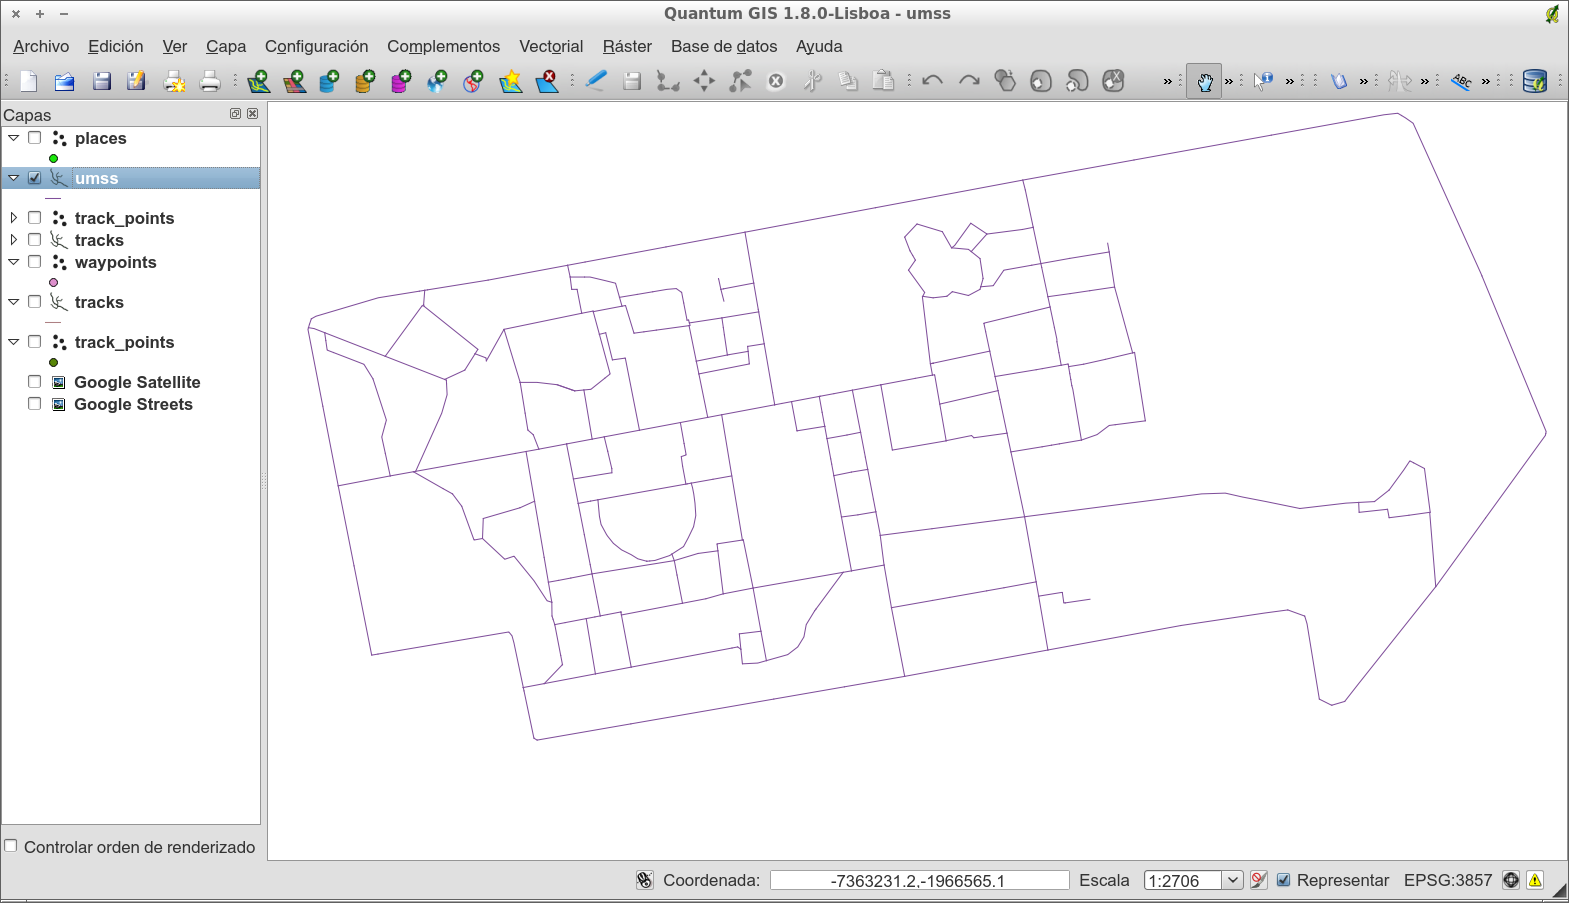
\includegraphics[width=0.8\textwidth]{rutas_qgis}
      \end{center}
      \caption{Rutas del Campus de la UMSS en QGis}
      \label{fig:rutas}
    \end{figure}

    El mapa generado con las rutas cumple con las caracteristicas de un grafo ponderado no-dirigido en el que el costo o peso de las aristas es la distacia entre los nodos y los nodos son los puntos de interseccion de las rutas. Por lo tanto se puede implentar el algoritmo de Dijkstra para encontrar el camino minimo.

  % section generacion_de_las_rutas (end)
  \section{Lectura de los archivos Shapefile} % (fold)
  \label{sec:lectura_de_los_archivos_shapefile}
    Es necesario cargar la base de datos PostGis con los shapefiles generados por QGis y para eso se uso la gema RGeo y con el siguiente metodo escrito en Ruby se carga los archivos shapefile en la base de datos.

    \begin{center}
      \begin{verbatim}
  def self.load_shapefile(path)
    RGeo::Shapefile::Reader.open(path, factory: FACTORY) do |file|
      file.each do |record|
        way = record.geometry.projection
        ruta = Way.create(name: record['id'], 
                          dist: way.length,  
                          the_geom: way[0])
      end
    end
  end
      \end{verbatim}
    \end{center}

  % section lectura_de_los_archivos_shapefile (end)
  \section{Los lugares} % (fold)
  \label{sec:los_lugares}
    Los lugares o sitios de interes se crean atraves de la aplicacion, ingresando a la seccion de \emph{Nuevo lugar}, en donde es necesario llenar el formulario y hacer un click sobre el mapa en el sitio que se desea registrat el nuevo lugar.

    \begin{figure}[!ht]
      \begin{center}
        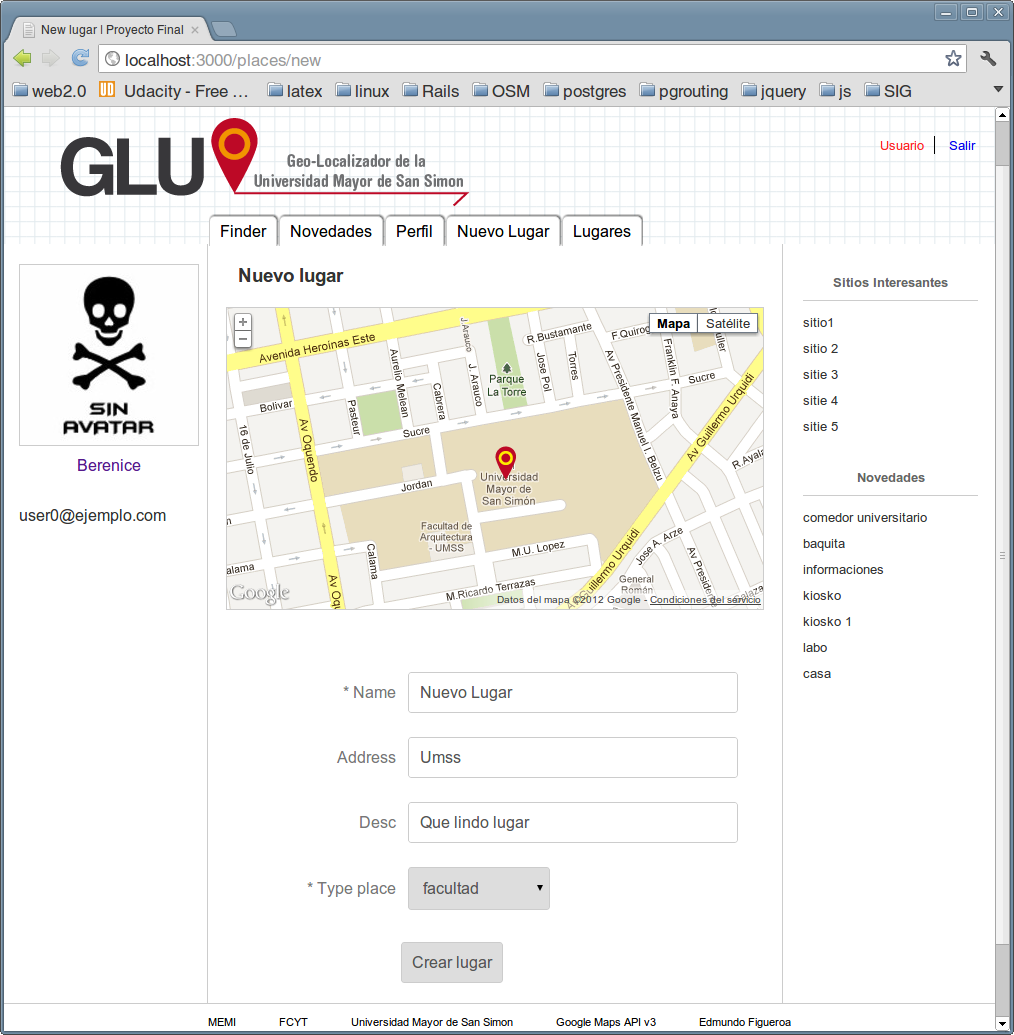
\includegraphics[width=0.8\textwidth]{new_place}
      \end{center}
      \caption{Registro de Nuevos lugares}
      \label{fig:new_place}
    \end{figure}
    % pero para fines practicos se registraron inicialmente unos 5x lugares mediante un shapefile 
    \subsection{La geolocalizacion de los lugares} % (fold)
    \label{subsec:la_geolocalizacion_de_los_lugares}
      % Como creo dentro de rails un lugar.
      Para que Rails cree un lugar es necesario los siguentes pasos: 
        \begin{itemize}
          \item Declarar un objeto que maneja la proyeci\'on \\
          \verb+ FACTORY = RGeo::Geographic.simple_mercator_factory +
          \item Declarar el atributo encargado de manejar el dato espacial, mediante el metodo \emph{set\_rgeo\_factory\_for\_column} especificando la proyeci\'on. \verb|set_rgeo_factory_for_column(:coord, FACTORY.projection_factory)|
          \item LLamar a al funcion \emph{create\_coord} cuando se crea un nuevo lugar, siempre teniendo en cuenta la proyecion en la cual se reciben los datos (\emph{lon} y \emph{lat} se reciben del lado del cliente en WS84) y proyectarlo para guardarlo correctamente en la base de datos (\emph{coord} esta en la proyecion EPSG 3785).
          % \begin{center}
          \begin{verbatim}
    def create_coord
      if self.new_record?
        self.coord = FACTORY.point(lon, lat).projection 
      else
        p self.coord
      end
    end
          \end{verbatim}
          % \end{center}
        \end{itemize}
        
    
    % section la_geolocalizacion_de_los_lugares (end)
  
  % section los_lugares (end)
  \section{Modelo de base de datos} % (fold)
  \label{sec:modelo_de_base_de_datos}
  
  % section modelo_de_base_de_datos (end)
  \section{Camino minimo} % (fold)
  \label{sec:camino_minimo}

    Una ves se tienen las rutas en la base de datos es necesario realizar algunos pasos previos para encontrar el camino minimo, pgRouting requiere de una tabla en la especifica todos los vertices existentes. Toma como argumentos la tabla de la cual se debe extraer los vertices (ways), la distancia de tolerancia (0.001), el atributo espacial (the\_geom) y su id (gid)

    \begin{center}
      \begin{verbatim}
      SELECT assign_vertex_id('ways', 0.001, 'the_geom', 'gid');
      \end{verbatim}
    \end{center}

    Al tener ya lista la base de datos, se procede a llamar a la funcion \emph{shortest\_path} del modulo PgRouting  de PostGis, el cual implementa el algoritmo de Dijkstra para encontrar el camino minimo. 

    En una computadora AMD K6 de 1.8 GHz, de 346 vertices se tiene el siguiente dato

    \begin{center}
      \begin{verbatim}
-- Executing query:
SELECT  * from  shortest_path('select gid as id, 
                              source::integer,
                              target::integer, 
                              dist::double precision as cost from ways',
                              20, 299 , 
                              false, false)
Total query runtime: 11 ms.
31 rows retrieved.
      \end{verbatim}
    \end{center}

    La funcion shortest\_path toma como variables el id del vertice origen (20), y el vertice destino (299).

  
  % section camino_minimo (end)

  \section{Modelos ?} % (fold)
  \label{sec:modelos_}
  
  % section modelos_ (end)
  \section{Diagrama de casos de uso ?} % (fold)
  \label{sec:diagrama_de_casos_de_uso_}
  
  % section diagrama_de_casos_de_uso_ (end)







% chapter descripcion_de_la_implentacion (end)


% la red social en la que los usuarios comparten las fotos de los sitios que visitan.
  % \include{pruebas}

\backmatter
  \begin{thebibliography}{99}
  \bibitem{awdr4e} Sam Ruby, Dave Thomas, David Heinemeier Hansson, \emph{Agile Web Development with Rails, Fourth Edition}
  \bibitem{web2}  http://trends.builtwith.com/topsites/Ruby-on-Rails
  \bibitem{web3} tumblr.yasulab.jp/post/10271634919/5-question-interview-with-twitter-developer-alex-payne
  \bibitem{web4} http://www.artima.com/scalazine/articles/twitter\_on\_scala.html
  \bibitem{web5} http://oreilly.com/web2/archive/what-is-web-20.html
  \bibitem{web9} http://radar.oreilly.com/2006/12/web-20-compact-definition-tryi.html
  \bibitem{web6} http://www.ics.uci.edu/~fielding/pubs/dissertation/top.htm
  \bibitem{web7} http://st-www.cs.illinois.edu/users/smarch/st-docs/mvc.html
  \bibitem{web8} http://msdn.microsoft.com/en-us/architecture/bb906060.aspx
  \bibitem{json} http://www.json.org/json-es.html
  \bibitem{coords} http://kartoweb.itc.nl/geometrics/Coordinate\%20systems/coordsys.html
  \bibitem{p_iscs} Introduction to Spatial Coordinate Systems: Flat Maps for a Round Planet,\\ http://msdn.microsoft.com/en-us/library/cc749633(v=sql.100).aspx
  \bibitem{projected_ibm} http://publib.boulder.ibm.com/infocenter/db2luw/v8/index.jsp?\\topic=/com.ibm.db2.udb.doc/opt/csb3022b.htm
  \bibitem{msdn_srid} http://msdn.microsoft.com/es-es/library/bb964707.aspx

\end{thebibliography}

  % \listoffigures
  % \listoftables
% \newpage
\end{document}
